 \documentclass[11pt]{article}  

%%%%%%%% PREÁMBULO %%%%%%%%%%%%
\title{CG}

\usepackage{tikz}
\usepackage[spanish]{babel} %Indica que escribiremos en español
\usepackage[utf8]{inputenc} %Indica qué codificación se está usando ISO-8859-1(latin1)  o utf8 
\usepackage{amsmath}
\usepackage{amssymb} % Símbolos matematicos (por lo tanto)
\usepackage{graphicx} % Incluir imágenes en LaTeX
\usepackage{color} % Para colorear texto
\usepackage{array}
\usepackage{multirow}
\usepackage{enumitem}
\usepackage{subcaption}
\usepackage{graphicx}
\usepackage{tabu}
\usepackage{listings} % Para usar código fuente
\usepackage{xcolor}

\definecolor{codegreen}{rgb}{0,0.6,0}
\definecolor{codegray}{rgb}{0.5,0.5,0.5}
\definecolor{codepurple}{rgb}{0.58,0,0.82}
\definecolor{backcolour}{rgb}{0.95,0.95,0.92}
\definecolor{lightgray}{rgb}{0.95, 0.95, 0.95}
\definecolor{darkgray}{rgb}{0.4, 0.4, 0.4}
%\definecolor{purple}{rgb}{0.65, 0.12, 0.82}
\definecolor{editorGray}{rgb}{0.95, 0.95, 0.95}
\definecolor{editorOcher}{rgb}{1, 0.5, 0} % #FF7F00 -> rgb(239, 169, 0)
\definecolor{editorGreen}{rgb}{0, 0.5, 0} % #007C00 -> rgb(0, 124, 0)
\definecolor{orange}{rgb}{1,0.45,0.13}		
\definecolor{olive}{rgb}{0.17,0.59,0.20}
\definecolor{brown}{rgb}{0.69,0.31,0.31}
\definecolor{purple}{rgb}{0.38,0.18,0.81}
\definecolor{lightblue}{rgb}{0.1,0.57,0.7}
\definecolor{lightred}{rgb}{1,0.4,0.5}

\lstdefinestyle{mystyle}{
    backgroundcolor=\color{backcolour},   
    commentstyle=\color{codegreen},
    keywordstyle=\color{magenta},
    numberstyle=\tiny\color{codegray},
    stringstyle=\color{codepurple},
    basicstyle=\ttfamily\footnotesize,
    breakatwhitespace=false,         
    breaklines=true,                 
    captionpos=b,                    
    keepspaces=true,                 
    numbers=left,                    
    numbersep=5pt,                  
    showspaces=false,                
    showstringspaces=false,
    showtabs=false,                  
    tabsize=2
}
% JavaScript
\lstdefinelanguage{JavaScript}{
  morekeywords={this, typeof, new, true, false, catch, function, return, null, catch, switch, var, if, in, while, do, else, case, break, let, const, :},
  morecomment=[s]{/*}{*/},
  morecomment=[l]//,
  morestring=[b]",
  morestring=[b]'
}

\lstdefinelanguage{HTML5}{
  language=html,
  sensitive=true,	
  alsoletter={<>=-},	
  morecomment=[s]{<!-}{-->},
  tag=[s],
  otherkeywords={
  % General
  >,
  % Standard tags
	<!DOCTYPE,
  </html, <html, <head, <title, </title, <style, </style, <link, </head, <meta, />,
	% body
	</body, <body,
	% Divs
	</div, <div, </div>, 
	% Paragraphs
	</p, <p, </p>,
	% scripts
	</script, <script,
  % More tags...
  <canvas, /canvas>, <svg, <rect, <animateTransform, </rect>, </svg>, <video, <source, <iframe, </iframe>, </video>, <image, </image>, <header, </header, <article, </article, <input,<button, </button, <label, </label, <br,/br>
  },
  ndkeywords={
  % General
  =,
  % HTML attributes
  charset=, src=, id=, width=, height=, style=, type=, rel=, href=,
  % SVG attributes
  fill=, attributeName=, begin=, dur=, from=, to=, poster=, controls=, x=, y=, repeatCount=, xlink:href=,
  % properties
  margin:, padding:, background-image:, border:, top:, left:, position:, width:, height:, margin-top:, margin-bottom:, font-size:, line-height:,
	% CSS3 properties
  transform:, -moz-transform:, -webkit-transform:,
  animation:, -webkit-animation:,
  transition:,  transition-duration:, transition-property:, transition-timing-function:,
  }
}
\lstdefinestyle{htmlcssjs} {%
  % General design
%  backgroundcolor=\color{editorGray},
  backgroundcolor=\color{backcolour},   
  basicstyle=\ttfamily\footnotesize,
  basicstyle={\footnotesize\ttfamily},   
  frame=b,
  % line-numbers
  xleftmargin={0.75cm},
  numbers=left,
  stepnumber=1,
  firstnumber=1,
  numberfirstline=true,	
  % Code design
  identifierstyle=\color{black},
  keywordstyle=\color{blue}\bfseries,
  ndkeywordstyle=\color{editorGreen}\bfseries,
  stringstyle=\color{editorOcher}\ttfamily,
  commentstyle=\color{brown}\ttfamily,
  % Code
  language=HTML5,
  alsolanguage=JavaScript,
  alsodigit={.:;},	
  tabsize=2,
  showtabs=false,
  showspaces=false,
  showstringspaces=false,
  extendedchars=true,
  breaklines=true,
  % German umlauts
  literate=%
  {Ö}{{\"O}}1
  {Ä}{{\"A}}1
  {Ü}{{\"U}}1
  {ß}{{\ss}}1
  {ü}{{\"u}}1
  {ä}{{\"a}}1
  {ö}{{\"o}}1
}


\lstset{style=mystyle}

\definecolor{dkgreen}{rgb}{0,0.6,0} % Definimos colores para usar en el código
\definecolor{gray}{rgb}{0.5,0.5,0.5} 
% configuración para el lenguaje que queramos utilizar
\lstset{language=Matlab,
   keywords={break,case,catch,continue,else,elseif,end,for,function,
      global,if,otherwise,persistent,return,switch,try,while},
   basicstyle=\ttfamily,
   keywordstyle=\color{blue},
   commentstyle=\color{red},
   stringstyle=\color{dkgreen},
   %numbers=left,
   %numberstyle=\tiny\color{gray},
   %stepnumber=1,
   numbersep=10pt,
   backgroundcolor=\color{white},
   tabsize=4,
   showspaces=false,
   showstringspaces=false}



\newcommand{\sen}{\operatorname{\sen}}	% Definimos el comando \sen para el seno
%en español

\usepackage{float} %Podemos usar el especificador [H] en las figuras para que se
% queden donde queramos
\usepackage{capt-of} % Permite usar etiquetas fuera de elementos flotantes
% (etiquetas de figuras)
\usepackage{sidecap} % Para poner el texto de las imágenes al lado
	\sidecaptionvpos{figure}{c} % Para que el texto se alinie al centro vertical
\usepackage{caption} % Para poder quitar numeracion de figuras
\usepackage{sidecap} % Para poner el texto de las imágenes al lado
	\sidecaptionvpos{figure}{c} % Para que el texto se alinie al centro vertical
\usepackage{caption} % Para poder quitar numeracion de figuras
\usepackage{commath} % funcionalidades extras para diferenciales,
\usepackage{commath} % funcionalidades extras para diferenciales, integrales,
% etc (\od, \dif, etc)
\usepackage{cancel} % para cancelar expresiones (\cancelto{0}{x})
\usepackage{subcaption}
 
\usepackage{anysize} 					% Para personalizar el anchhttps://www.overleaf.com/project/5c0fb40aa77c632fc1f86e58o de  los márgenes
\marginsize{2cm}{2cm}{2cm}{2cm} % Izquierda, derecha, arriba, abajo

\usepackage{appendix}
\renewcommand{\appendixname}{Apéndices}
\renewcommand{\appendixtocname}{Apéndices}
\renewcommand{\appendixpagename}{Apéndices} 

% Para que las referencias sean hipervínculos a las figuras o ecuaciones y
% aparezcan en color
\usepackage[colorlinks=true,plainpages=true,citecolor=blue,linkcolor=blue]{hyperref}
%\usepackage{hyperref} 
% Para agregar encabezado y pie de página
\usepackage{fancyhdr} 
\pagestyle{fancy}
\fancyhf{}
\fancyhead[L]{\footnotesize UNSA} %encabezado izquierda
\fancyhead[R]{\footnotesize EPCC}   % dereecha
\fancyfoot[R]{\footnotesize CG}  % Pie derecha
\fancyfoot[C]{\thepage}  % centro
\fancyfoot[L]{\footnotesize Ciencia de la Computación}  %izquierda


\title{Trabajo}

%%%%%%%% TERMINA PREÁMBULO %%%%%%%%%%%%

\begin{document}

%%%%%%%%%%%%%%%%%%%%%%%%%%%%%%%%%% PORTADA %%%%%%%%%%%%%%%%%%%%%%%%%%%%%%%%%%%%%%%%%%%%
																					%%%
\begin{center}																		%%%
\newcommand{\HRule}{\rule{\linewidth}{0.5mm}}									%%%\left
 																					%%%
\begin{minipage}{0.5\textwidth} \begin{flushleft}

\includegraphics[scale = 0.4]{img/cslogo.png}
\end{flushleft}\end{minipage}
\begin{minipage}{0.48\textwidth} \begin{flushright}

\includegraphics[scale = 0.3]{img/logounsa.png}
\end{flushright}\end{minipage}

													 								%%%
\vspace*{-1.5cm}								%%%
																					%%%	
\textsc{\huge UNIVERSIDAD NACIONAL DE\\ SAN AGUSTÍN \vspace{5px}}\\[1.5cm]	

\textsc{\LARGE Facultad de Ingeniería de Producción y Servicios}\\[1.5cm]													%%%

\begin{minipage}{0.9\textwidth} 
\begin{center}																					%%%
\textsc{\LARGE Ciencia de la Computación}
\end{center}
\end{minipage}\\[0.5cm]
%%%
    																				%%%
 			\vspace*{1cm}																		%%%
																					%%%
\HRule \\[0.4cm]																	%%%
{ \huge \bfseries Laboratorio 1
}\\[0.4cm]	%%%
 																					%%%
\HRule \\[1.5cm]																	%%%
 																				%%%
																					%%%
\begin{minipage}{0.46\textwidth}													%%%
\begin{flushleft} \large															%%%
\centering

\textbf{ALUMNOS:}\\
Pfuturi Huisa, Oscar David\\
Quispe Menor, Hermogenes\\
Quiñonez Lopez, Efrain German\\
Fernandez Mamani, Brayan Gino\\
Santos Apaza, Yordy Williams

\	\vfill

\textbf{DOCENTE:} \\
MSc. Vicente Machaca Arceda

\	\vfill

\textbf{CURSO:}\\
Computación Gráfica

%\vspace*{2cm}	
            													%%%
										 						%%%
\end{flushleft}																		%%%
\end{minipage}		
																%%%
\begin{minipage}{0.70\textwidth}		
\vspace{-0.6cm}											%%%
																	%%%
\end{minipage}	
\vspace*{1cm}
%\begin{flushleft}
 	
%\end{flushleft}
%%%																		%%%
\vspace{3cm} 																				
\begin{center}																					
{\large \today}																	%%%
 			\end{center}												  						
\end{center}							 								\newpage
\newpage																

\tableofcontents 

\newpage
%%%%%%%%%%%%%%%%%%%%%%%%%%%%%%%%%%%%%%%%%%%%%%%%%%%%%%%%%%%%%%%%
\section{Github}

\begin{itemize}
    \item \url{https://github.com/oscar-pfuturi-h/Comp-Grafica}
\end{itemize}

\section{Funciones}
En el archivo helpers.py se agruparon las principales funciones, tenemos las funciones básicas cube, cone, sphere las cuales configuramos los tamaños de los objetos tanto en los 3 ejes(X, Y, Z)
\begin{lstlisting}[language=python,frame=single]
def cube(size_x, size_y, size_z):
    cube_shape = vtk.vtkCubeSource()
    cube_shape.SetXLength(size_x)
    cube_shape.SetYLength(size_y)
    cube_shape.SetZLength(size_z)
    cube_shape.Update()
    mapp_object = vtk.vtkPolyDataMapper()
    mapp_object.SetInputData(cube_shape.GetOutput())
    return mapp_object

def cone(radius,height,resolution):
    cone_shape = vtk.vtkConeSource()
    ...
    return mapp_object

def sphere(radius):
    sphere_shape = vtk.vtkSphereSource()
    ...
    return mapp_object
\end{lstlisting}

La función actor es la que se encarga de recibir los mappers de los objetos básicos y luego dependiendo de los diferentes parámetros se empieza a personalizar, como ejemplo posición en el plano, ángulos de rotación, color o texturas, al final nos devolverá objetos tipo actor para poder ser agregados al render.
\begin{lstlisting}[language=python,frame=single]
def actor(mapper,xyz,angle,rgb,texture_name):
    actor = vtk.vtkActor()
    #Cargar Texturas
    if texture_name is not None:
        reader = vtk.vtkJPEGReader()
        reader.SetFileName(texture_name)
        texture = vtk.vtkTexture()
        if vtk.VTK_MAJOR_VERSION <= 5:
            texture.SetInput(reader.GetOutput())
        else:
            texture.SetInputConnection(reader.GetOutputPort())
        actor.SetTexture(texture)
    if rgb is not None:
        actor.GetProperty().SetColor(transformRGBRange(rgb))
    if angle[0] is not None:
        actor.RotateX(angle[0])
    if angle[1] is not None:
        actor.RotateY(angle[1])
    if angle[2] is not None:
        actor.RotateZ(angle[2])
    actor.SetMapper(mapper)
    actor.SetPosition(xyz)
    return actor
\end{lstlisting}

En el caso de que requiera que se creen varios actores, se crearon funciones auxiliares como por ejemplo la creación de vallas.

\begin{lstlisting}[language=python,frame=single]
def crearVallas(cubos,color,angle,xyz,cantidad,tamx,tamz):
    vallas = []
    tam1 = tamx
    tam2 = tamz
    for i in range(cantidad):
        cActor1 = createActor(cubos[0],color,angle,[xyz[0]-tamx,xyz[1],xyz[2]-tamz])
        cActor2 = createActor(cubos[1],color,angle,[xyz[0]-tamx,xyz[1],xyz[2]-tamz])
        cActor3 = createActor(cubos[2],color,angle,[xyz[0]-tamx,xyz[1],xyz[2]-tamz])
        cActor4 = createActor(cubos[3],color,angle,[xyz[0]-tamx,xyz[1],xyz[2]-tamz])
        tamx = tamx+tam1
        tamz = tamz+tam2
        vallas.append(cActor1)
        vallas.append(cActor2)
        vallas.append(cActor3)
        vallas.append(cActor4)
    return vallas

\end{lstlisting}

Se creo un función auxiliar en el caso de que se quieran agregar muchos Actores al renderer.


\begin{lstlisting}[language=python,frame=single]
def addActores(renderer,Actores):
    for i in Actores:
        renderer.AddActor(i)
\end{lstlisting}

\begin{lstlisting}[language=python,frame=single]
vallas=crearVallas(cubos,[255, 225, 53],[0,90,None],[36,0,78],9,8,0)
addActores(renderer,vallas)
\end{lstlisting}


\section{Resultados}
En el trabajo realizado se creo una granja. Para armar objetos como molino o animales se siguió la siguiente estructura, la cual nos permite configurar la mayoría de cosas en una simple linea de código.
\begin{lstlisting}[language=python,frame=single]
#-ACTORS(mapper/[position]/[angle]/[color]/texture_name)
act_techo=actor(techo,[20,14,20],[None,None,90],[219, 172, 121],None)
act_body=actor(body,[20,8,20],[None,None,90],[209, 204, 190],None)
act_aspa1=actor(aspa,[20,16,26],[None,None,None],[163, 130, 93],None)
act_aspa2=actor(aspa, [20,16,26], [None,None,90], [163, 130, 93],None)
act_estaca=actor(estaca,[20,16,23],[None,None,90],[163, 130, 93],None)
\end{lstlisting}
\begin{figure}[H]
    \centering    
    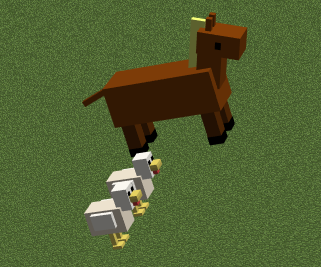
\includegraphics[scale=0.8]{img/anaimales.PNG}
    \caption{Patos y caballo}
\end{figure}

\begin{figure}[H]
    \centering    
    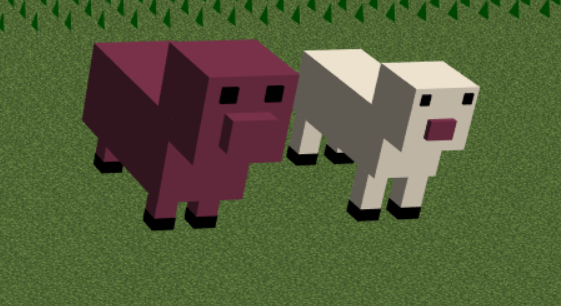
\includegraphics[scale=0.8]{img/cerdoYovejaF.png}
    \caption{cerdo y oveja}
\end{figure}

\begin{figure}[H]
    \centering    
    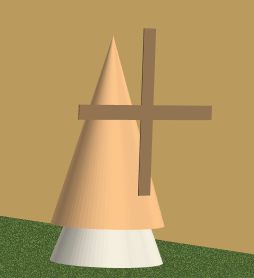
\includegraphics[scale=0.8]{img/molino.PNG}
    \caption{Molino}
\end{figure}
\begin{figure}[H]
    \centering    
    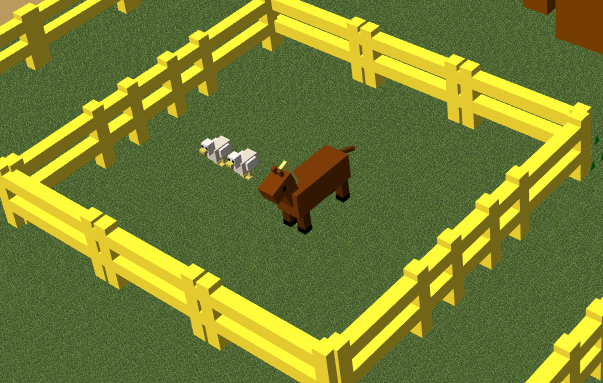
\includegraphics[scale=0.45]{img/vallas.png}
    \caption{Vallas}
\end{figure}
\begin{figure}[H]
    \centering    
    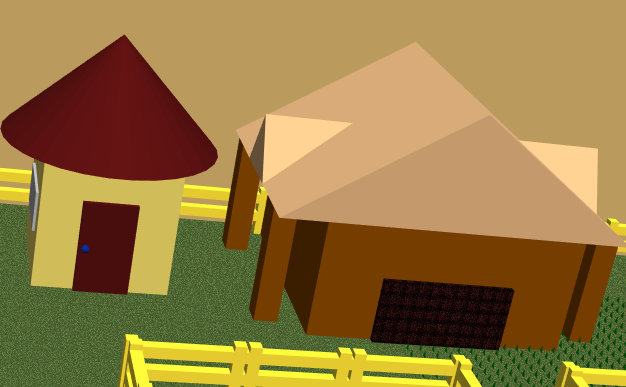
\includegraphics[scale=0.45]{img/casa-granero.png}
    \caption{Casa y granero}
\end{figure}
\begin{figure}[H]
    \centering    
    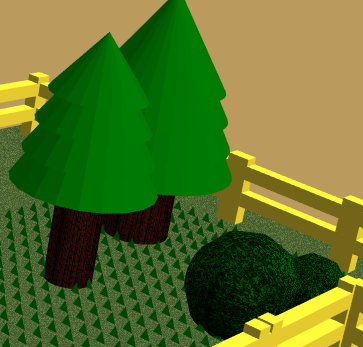
\includegraphics[scale=0.5]{img/vegetacion.png}
    \caption{Vegetación}
\end{figure}
\end{document}